\section{Experiment}
\label{sec:Experiment}

In accordance with existing multimodal out-of-context misinformation detection methods \cite{abdelnabi2022open, qi2024sniffer}, we conduct a multitude of experiments to demonstrate the effectiveness of the proposed E2LVLM on the public benchmark dataset NewsCLIPpings~\cite{luo2021newsclippings}. Typically, we focus on the six evaluation questions as follows:
\begin{enumerate}[label=\textbf{Q\arabic*:}]
    \item  How does E2LVLM perform in the task of multimodal OOC misinformation detection?
    \item  How does each procedure contribute to the E2LVLM's performance in detection?
    \item  Does E2LVLM provide accurate detections and compelling rationales for their judgments?
    \item  How impact are different sizes of the base LVLM on E2LVLM in detection?
    \item  Can E2LVLM be rapidly deployed at the stage of early detection?
    \item  How does E2LVLM perform on the other dataset?
\end{enumerate}

\subsection{Experimental Setup}

\textbf{Dataset.} We evaluate the efficacy of the proposed E2LVLM on the dataset NewsCLIPpings~\cite{luo2021newsclippings}. This dataset serves as the largest real-world multimodal misinformation detection benchmark. We follow the standard protocol \cite{abdelnabi2022open, yuan2023support, qi2024sniffer}, and report experimental results on the Merged/Balance subset. This subset consists of 71,072 training, 7,024 validation, and 7,264 testing, respectively.

\noindent \textbf{Compared Baselines.} To make a comprehensive performance evaluation, we compare the proposed E2LVLM with a series of representative methods. (1) A line of research focuses on attached classifiers trained from scratch, including SAFE~\cite{massarelli2019safe} and EANN~\cite{wang2018eann}. (2) Another line of research underlines the use of pre-trained models, containing VisualBERT~\cite{li2019visualbert}, CLIP~\cite{radford2021learning}, Neu-Sym detector~\cite{zhang2023detecting}, DT-Transformer~\cite{papadopoulos2023synthetic}, CCN~\cite{abdelnabi2022open}, SEN~\cite{yuan2023support}, and ECENet~\cite{zhang2023ecenet}. (3) Furthermore, in the era of LVLMs, SNIFFER~\cite{qi2024sniffer} is the first attempt to adopt a multimodal large language model for addressing the OOC task. More details of these methods can be provided in their official papers. 

\noindent \textbf{Evaluation Metrics.} We regard the multimodal OOC misinformation detection issue as a binary classification task. Following the standard process~\cite{abdelnabi2022open}, the accuracy over all samples (All), the accuracy over the OOC (Falsified), and not OOC (Pristine) are reported as the metrics during evaluation for a fair comparison.

\noindent \textbf{Implementation Details.} We choose Qwen2-VL-7B~\cite{wang2024qwen2} as the base LVLM, unless otherwise specified. We implement E2LVLM on PyTorch~\cite{paszke2019pytorch} version 2.3.1 with CUDA 12.2, and train it for 2 epochs on 4 NVIDIA GeForce RTX 3090 GPUs with 24G of memory. We adopt FlashAttention - 2~\cite{dao2024flashattention} for efficient training on the visual encoder and large language model. We use a batch size of 8 and a learning rate of $2\times 10^{-4}$. The models are optimized using AdamW~\cite{loshchilov2017decoupled} optimizer with a linear warmup and a cosine learning rate scheduler. Additionally, all experimental results are the average of three runs with no hyper-parameter searching.

% \clearpage
\subsection{RQ1: Comparison with SOTA Methods}

%-------------main results
% \begin{table}[t]
% \newcommand{\hlinebold}{\noalign{\hrule height 0.2mm}}
% \centering
% \caption{Performance for accuracy compared to existing OOC methods on the benchmark dataset NewsCLIPpings~\cite{luo2021newsclippings}. The best performances are indicated in \textbf{bold}.}
% \resizebox{\columnwidth}{!}{%
% \begin{tabular}{l|c|ccc}
% % \toprule
% Methods & Venue & \textbf{All} & \textbf{Falsified} & \textbf{Pristine}  \\
% \hlinebold
% SAFE~\cite{massarelli2019safe}  & PAKDD20 & 52.8 & 54.8 & 52.0  \\
% EANN~\cite{wang2018eann}  & SIGKDD18 & 58.1 & 61.8 & 56.2  \\
% \hline
% VisualBERT~\cite{li2019visualbert}  & arXiv19 & 58.6 & 38.9 & 78.4 \\
% CLIP~\cite{radford2021learning} & ICML21  & 66.0 & 64.3 & 67.7  \\
% Neu-Sym detector~\cite{zhang2023detecting} & arXiv23 & 68.2 & - & - \\
% DT-Transformer~\cite{papadopoulos2023synthetic} & MAD23 & 77.1 & 78.6 & 75.6  \\
% CCN~\cite{abdelnabi2022open} & CVPR22 & 84.7 & 84.8 & 84.5  \\
% SEN~\cite{yuan2023support} & EMNLP23 & 87.1 & 85.5 & 88.6  \\
% ECENet~\cite{zhang2023ecenet} & MM23 & 87.7 & - & - \\
% \hline
% SNIFFER~\cite{qi2024sniffer} & CVPR24 & 88.4 & 86.9 & \textbf{91.8}  \\
% \rowcolor{lightgreen} E2LVLM (\textit{Ours}) & & \textbf{89.9} & \textbf{90.3} & 89.4  \\
% % \hlinebold
% % \bottomrule
% \end{tabular}%
% }
% \label{tab:tab_1}
% \end{table}


% \begin{table}[t]
% \newcommand{\hlinebold}{\noalign{\hrule height 0.2mm}}
% \centering
% \small
% \caption{Performance for accuracy compared to existing OOC methods on the benchmark dataset NewsCLIPpings~\cite{luo2021newsclippings}. The best performances are indicated in \textbf{bold}.}
% \begin{adjustbox}{valign=c,max width=\columnwidth}
% \begin{tabular}{l|c|ccc}
% Methods & Venue & \textbf{All} & \textbf{Falsified} & \textbf{Pristine}  \\
% \hlinebold
% SAFE~\cite{massarelli2019safe}  & PAKDD20 & 52.8 & 54.8 & 52.0  \\
% EANN~\cite{wang2018eann}  & SIGKDD18 & 58.1 & 61.8 & 56.2  \\
% \hline
% VisualBERT~\cite{li2019visualbert}  & arXiv19 & 58.6 & 38.9 & 78.4 \\
% CLIP~\cite{radford2021learning} & ICML21  & 66.0 & 64.3 & 67.7  \\
% Neu-Sym detector~\cite{zhang2023detecting} & arXiv23 & 68.2 & - & - \\
% DT-Transformer~\cite{papadopoulos2023synthetic} & MAD23 & 77.1 & 78.6 & 75.6  \\
% CCN~\cite{abdelnabi2022open} & CVPR22 & 84.7 & 84.8 & 84.5  \\
% SEN~\cite{yuan2023support} & EMNLP23 & 87.1 & 85.5 & 88.6  \\
% ECENet~\cite{zhang2023ecenet} & MM23 & 87.7 & - & - \\
% \hline
% SNIFFER~\cite{qi2024sniffer} & CVPR24 & 88.4 & 86.9 & \textbf{91.8}  \\
% \rowcolor{lightgreen} E2LVLM (\textit{Ours}) & & \textbf{89.9} & \textbf{90.3} & 89.4  \\
% \end{tabular}%
% \end{adjustbox}
% \label{tab:tab_1}
% \end{table}

\Cref{tab:tab_1} presents the detailed comparison of E2LVLM with existing OOC methods on NewsCLIPpings. We use ``-'' for partial methods that do not release source codes or results. As shown in these results, we summarize the following findings: (1) As for the accuracy over ``All'', E2LVLM outperforms all methods by a large margin. Even for the state-of-the-art (SNIFFER), E2LVLM still outperforms it by around 1.5\% accuracy. (2) E2LVLM owns strong discriminatory powers, with an improvement of around 3.4\% over ``Falsified'', increasing the SOTA from 86.9\% to 90.3\%. (3) E2LVLM has a trade-off between ``Falsified'' and ``Pristine''. As reported by CCN~\cite{abdelnabi2022open}, a professional OOC misinformation detector should accurately identify both ``Falsified'' and ``Pristine'' samples. E2LVLM provides a closer distance between them, compared with the SOTA. This confirms that the improvement in the E2LVLM's performance on ``Falsified'' does not come at the cost of its performance on ``Pristine'', or vice versa. (4) With the increasing of architectural complexity, the performance of OOC misinformation detectors has been significantly enhanced, which is consistent with previous statements. In the context of LVLMs-based OOC methods, E2LVLM with Qwen2-VL-7B~\cite{wang2024qwen2} is superior to SNIFFER that depends on GPT-4~\cite{achiam2023gpt} and Vicuna-13B~\cite{vicuna2023}. These findings suggest the superiority of the proposed method E2LVLM on the OOC detection.


\begin{table}[t]
    \caption{Performance for accuracy compared to existing methods on NewsCLIPpings~\cite{luo2021newsclippings}. The best results are indicated in \textbf{bold}.}
      \centering
      \begin{adjustbox}{valign=c, max width=\columnwidth}
      \begin{tabular}{l|c|ccc}
        \toprule
        Methods & Venue & \textbf{All} & \textbf{Falsified} & \textbf{Pristine}  \\
        \hline
        SAFE~\cite{massarelli2019safe}  & PAKDD20 & 52.8 & 54.8 & 52.0  \\
        EANN~\cite{wang2018eann}  & SIGKDD18 & 58.1 & 61.8 & 56.2  \\
        \hline
        VisualBERT~\cite{li2019visualbert}  & arXiv19 & 58.6 & 38.9 & 78.4 \\
        CLIP~\cite{radford2021learning} & ICML21  & 66.0 & 64.3 & 67.7  \\
        Neu-Sym detector~\cite{zhang2023detecting} & arXiv23 & 68.2 & - & - \\
        DT-Transformer~\cite{papadopoulos2023synthetic} & MAD23 & 77.1 & 78.6 & 75.6  \\
        CCN~\cite{abdelnabi2022open} & CVPR22 & 84.7 & 84.8 & 84.5  \\
        SEN~\cite{yuan2023support} & EMNLP23 & 87.1 & 85.5 & 88.6  \\
        ECENet~\cite{zhang2023ecenet} & MM23 & 87.7 & - & - \\
        \hline
        SNIFFER~\cite{qi2024sniffer} & CVPR24 & 88.4 & 86.9 & \textbf{91.8}  \\
        \rowcolor{lightgreen} E2LVLM (\textit{Ours}) & & \textbf{89.9} & \textbf{90.3} & 89.4  \\
        \bottomrule
  \end{tabular}
  \end{adjustbox}
  \label{tab:tab_1}
\end{table}



% %------------------main results
% \begin{table}[t]
% \newcommand{\hlinebold}{\noalign{\hrule height 0.2mm}}
% \centering
% \small
% \caption{Performance for accuracy compared to existing OOC methods on the benchmark dataset NewsCLIPpings~\cite{luo2021newsclippings}. The best performances are indicated in \textbf{bold}.}
% \begin{adjustbox}{valign=c,max width=\columnwidth}
% \begin{tabular}{l|c|ccc}
% \toprule
% Methods & Venue & \textbf{All} & \textbf{Falsified} & \textbf{Pristine}  \\
% \hlinebold
% SAFE~\cite{massarelli2019safe}  & PAKDD20 & 52.8 & 54.8 & 52.0  \\
% EANN~\cite{wang2018eann}  & SIGKDD18 & 58.1 & 61.8 & 56.2  \\
% \hline
% VisualBERT~\cite{li2019visualbert}  & arXiv19 & 58.6 & 38.9 & 78.4 \\
% CLIP~\cite{radford2021learning} & ICML21  & 66.0 & 64.3 & 67.7  \\
% Neu-Sym detector~\cite{zhang2023detecting} & arXiv23 & 68.2 & - & - \\
% DT-Transformer~\cite{papadopoulos2023synthetic} & MAD23 & 77.1 & 78.6 & 75.6  \\
% CCN~\cite{abdelnabi2022open} & CVPR22 & 84.7 & 84.8 & 84.5  \\
% SEN~\cite{yuan2023support} & EMNLP23 & 87.1 & 85.5 & 88.6  \\
% ECENet~\cite{zhang2023ecenet} & MM23 & 87.7 & - & - \\
% \hline
% SNIFFER~\cite{qi2024sniffer} & CVPR24 & 88.4 & 86.9 & \textbf{91.8}  \\
% \rowcolor{lightgreen} E2LVLM (\textit{Ours}) & & \textbf{89.9} & \textbf{90.3} & 89.4  \\
% \end{tabular}%
% \end{adjustbox}
% \label{tab:tab_1}
% \end{table}
% \clearpage
\subsection{RQ2: Ablation Study}

\begin{table}[t]
\caption{Ablation experiments for the E2LVLM. Evaluated on the NewsCLIPpings~\cite{luo2021newsclippings}. ``\#Evid.'' and ``\#Expla.'' represent the use of textual evidence and the supervised signal with explanations.}
\centering
\setlength{\tabcolsep}{1.5pt} % 调整列间距,减小为4pt
\renewcommand{\arraystretch}{1.2} % 调整行高(默认为1)
    \begin{adjustbox}{valign=c,max width=\columnwidth}
        \begin{tabular}{cccccc|ccc}
            \toprule
            Qwen2-VL & \#Evid. & Rerank & Rewrite& \#Expla. & Tuning & \textbf{All} & \textbf{Falsified} & \textbf{Pristine} \\
            \hline
            \cmark & \xmark & \xmark & \xmark & \xmark &\xmark & 69.1 & 54.4 & 83.9 \\
            \cmark & \cmark & \xmark & \xmark & \xmark &\xmark & 76.7 &	68.0 &	85.3 \\
            \hline
            \cmark & \xmark & \xmark & \xmark & \xmark &\cmark   & 78.9 & 73.8 & 84.2 \\
            \cmark & \cmark & \xmark & \xmark & \xmark &\cmark   & 83.0 & 77.1 & 88.9 \\
            \cmark & \cmark & \cmark & \xmark & \xmark &\cmark   & 87.7 & 86.5 & 88.7  \\
            \cmark & \cmark & \cmark & \cmark & \xmark &\cmark   & 88.5 & 87.7 & 89.1  \\
            \rowcolor{lightgreen} \cmark & \cmark & \cmark & \cmark &  \cmark &\cmark  & \textbf{89.9} & \textbf{90.3} & \textbf{89.4} \\
            \bottomrule
        \end{tabular}
    \end{adjustbox}
\label{tab:tab_2}
\end{table}









We conduct ablation experiments to analyze the effectiveness of primary procedures in E2LVLM. The results are shown in \Cref{tab:tab_2}, we can obtain the following findings:

\begin{itemize}
    \item We evaluate the impact of the use of textual evidence in zero-shot scenarios. As shown in the first two rows of \Cref{tab:tab_2}, the introduction of evidence achieves significant gains in performance, especially over ``Falsified''. Typically, the raw Qwen2-VL~\cite{wang2024qwen2} provides an accuracy of 69.1$\%$ over ``All'', which is higher than random guessing. It is attributed to the multimodal understanding capabilities of LVLMs. However, the base model struggles to discern falsified information, which necessitates robust methods to handle this challenge. Introducing textual evidence into the base model provides a performance improvement of 13.6$\%$ over the OOC. Besides, the accuracy on ``All'' reaches 76.7$\%$ (a 7.6$\%$ improvement in performance). This suggests the importance of the use of textual evidence in LVLMs for the OOC detection.
    \item In the second study, as shown in the remainder of \Cref{tab:tab_2}, each procedure contributes to the performance of E2LVLM. Typically, the task-specific fine-tuning technology extends LVLMs to the OOC, leading to promising results compared with zero-shot scenarios. Next, we conduct the textual evidence reranking strategy on E2LVLM, focusing on the salient item for debunking OOC misinformation. This results in an accuracy of 87.7$\%$ on ``All'', and shows a 9.4$\%$ improvement on ``Falsified'', while avoiding performance degradation on ``Pristine''. The reason is that such strategy appropriately eliminates the noise in the retrieved evidence. Further, we enforce the textual evidence rewriting strategy to generate coherent and contextually attuned content for better understanding, leading to an accuracy of 88.5$\%$ on ``All''. This suggests the importance of the reranking and rewriting of the retrieved textual evidence in E2LVLM for the OOC detection.
    \item Additionally, to understand the importance of the model’s explainability, we introduce the supervised signal with both judgment and explanation to the training phase, as shown in the last row of \Cref{tab:tab_2}. This results in an accuracy of 90.3$\%$ over ``Falsified'', higher than others. This is caused by the fact that such supervised signal enhances the model's discriminatory powers, thereby making the model provide accurate detections and attach them with compelling rationales for judgments. These results indicate that the supervised signal with both judgment and explanation contributes to the performance of E2LVLM.
\end{itemize}

% \newpage




\subsection{RQ3: Detection and Beyond}

%---------------------------------
% \begin{figure}[t]
%   \centering
%     \fbox{\rule{0pt}{1.8in} \rule{.8\linewidth}{0pt}}
%    \caption{Reranking performance of E2LVLM.  }
%    \label{fig:4}
% \end{figure}

\begin{figure}[t]
  \centering
   \includegraphics[width=.9\linewidth]{fig4.jpg}
   \caption{Comparison of E2LVLM with various reranking ways.}
   \label{fig:4}
\end{figure}

% \begin{figure}[t]
%   \centering
%    \includegraphics[width=1\linewidth]{sec/fig5.jpg}
%    \caption{Visualization of various data distributions.}
%    \label{fig:5}
% \end{figure}


Considering authentic images in the OOC realm, we further evaluate the effectiveness of the textual evidence reranking and rewriting in E2LVLM for detection and beyond. In subsequent experiments, we uniformly adopt the accuracy over ``All'' samples for comparison, unless otherwise specified.

\noindent \textbf{Reranking Analysis.} Upon analysis experiments above, we have observed a significant performance of E2LVLM in the top-1 textual evidence. To understand the impact of this design, we start an investigation of E2LVLM's predictions, as shown in \Cref{fig:4}. We add other reranking ways for comparison, \ie, cosine similarity and random choice. For $k$, we set the range of it as $\{1,2,3\}$. As shown in these results, we can note that the change trends of accuracy are generally consistent across distinct ways, presenting degradations as the growth of textual evidence. This is caused by the fact that not all textual evidence is effective. This necessitates the textual evidence reranking to prevent the introduction of irrelevant items. Further, these results suggest that E2LVLM lies in the multimodal understanding and reranking capabilities of LVLMs, serving as a professional OOC misinformation detector that incorporates internal and external information for revealing misinformation.

\begin{figure}[t]
  \centering
   \includegraphics[width=1\linewidth]{fig5.jpg}
   \caption{Visualization of various data distributions.}
   \label{fig:5}
\end{figure}

\noindent \textbf{Explainability Analysis.} To illustrate the E2LVLM's explainability, we conduct a qualitative analysis around data distributions to comprehend the decision-making phase, as shown in \Cref{fig:5}. From the results, the following findings are drawn: 1) As for an image-claim pair with ``Falsified'' in subfigure (a) of \Cref{fig:5}, the authentic image and its rewritten content are far from the falsified claim. Simultaneously, the rewritten content is closer to the authentic image, which supports it and refutes its claim. This makes the proposed E2LVLM provide an accurate decision. 2) As for an image-claim pair with ``Pristine'' in subfigure (b) of \Cref{fig:5}, the representation distributions of the authentic image, rewritten content, and claim are close together. This promotes E2LVLM to accurately discern this sample. These cases indicate that E2LVLM can effectively provide both judgment and explanation for debunking OOC misinformation.

\subsection{RQ4: Discussion of Different LVLMs}




% \begin{table}[t]
% \caption{A multimodal OOC misinformation detectors in distinct settings. Evaluated on NewsCLIPpings~\cite{luo2021newsclippings}. ``\#Params.'' refers to the parameters of Large Language Models in LVLMs.}
% \centering
% % \setlength{\tabcolsep}{4pt} % 调整列间距,减小为4pt
% \renewcommand{\arraystretch}{1.1} % 调整行高(默认为1)
%     \begin{adjustbox}{valign=c,max width=\columnwidth}
%         \begin{tabular}{lc|c|ccc}
%             \toprule
%             Settings & Tuning& \#Params. & \textbf{All} & \textbf{Falsified} & \textbf{Pristine} \\
%             \hline
%             Random & \xmark & -  & 50.3	& 49.2 & 51.5 \\
%             Qwen2-VL-2B & \xmark & 1.5B  & 65.7 & 88.6 & 42.9 \\
%             Qwen2-VL-7B & \xmark & 7.6B  &  79.1 & 75.7  & 82.5  \\
%             Qwen2-VL-72B & \xmark & 72B  & 79.8 & 87.2 & 72.5  \\
%             \hline
%             Qwen2-VL-2B & \cmark & 1.5B  & 81.4	& 80.2 & 82.6 \\
%             \rowcolor{lightgreen} Qwen2-VL-7B & \cmark & 7.6B  & 89.9	& 90.3 &89.4 \\
%             \bottomrule
%         \end{tabular}
%     \end{adjustbox}
% \label{tab:tab_4}
% \end{table}


% \begin{table}[t]
% \caption{A multimodal OOC misinformation detectors with distinct LVLMs. Evaluated on the NewsCLIPpings~\cite{luo2021newsclippings} dataset.}
% \centering
% \small
% % \setlength{\tabcolsep}{0.5pt} % 调整列间距,减小为4pt
% % \renewcommand{\arraystretch}{1.1} % 调整行高(默认为1)
%     \begin{adjustbox}{valign=c,max width=\columnwidth}
%         \begin{tabular}{lc|c|c}
%             \toprule
%             Settings & Tuning & Parameters & \textbf{All} \\
%             \hline
%             Random & \xmark & -  & 50.3	\\
%             Qwen2-VL-2B & \xmark & 1.5B  & 65.7 \\
%             Qwen2-VL-7B & \xmark & 7.6B  &  79.1 \\
%             Qwen2-VL-72B & \xmark & 72B  & 79.8 \\
%             \hline
%             Qwen2-VL-2B & \cmark & 1.5B  & 81.4	\\
%             \rowcolor{lightgreen} Qwen2-VL-7B & \cmark & 7.6B  & \textbf{89.9} \\
%             \bottomrule
%         \end{tabular}
%     \end{adjustbox}
% \label{tab:tab_4}
% \end{table}


% \begin{table}[t]
% \caption{Performance comparison on distinct LVLMs between instructional data construction and model tuning. Evaluated on the NewsCLIPpings~\cite{luo2021newsclippings} dataset.}
% \centering
% \small
% % \setlength{\tabcolsep}{5.5pt} % 调整列间距,减小为4pt
% % \renewcommand{\arraystretch}{1.1} % 调整行高(默认为1)
%     \begin{adjustbox}{valign=c,max width=\columnwidth}
%         \begin{tabular}{lcl|c}
%         \toprule
%          Data Construction &  \ding{223} & Model  Tuning & \textbf{All} \\
%         \hline
%         Qwen2-VL-2B & \ding{223} & Qwen2-VL-2B   & 81.1 \\
%         Qwen2-VL-2B & \ding{223} & Qwen2-VL-7B   & 87.6 \\
%         \hline
%         Qwen2-VL-7B & \ding{223} & Qwen2-VL-2B   & 81.4 \\
%         \rowcolor{lightgreen} Qwen2-VL-7B & \ding{223} & Qwen2-VL-7B   & \textbf{89.9} \\
%         \bottomrule
%         \end{tabular}
%     \end{adjustbox}
% \label{tab:tab_5}
% \end{table}

To analyze the impact of distinct LVLMs on E2LVLM in the OOC detection, we conduct analysis experiments around Qwen2-VL family~\cite{wang2024qwen2} in \Cref{tab:tab_4} and \Cref{tab:tab_5}. As depicted in these results, we achieve the following observations:



% The former is to evaluate the impact of the chosen base LVLM during training, and the latter is to measure the mutual synergy between instructional data construction and model tuning. 

(1) As shown in \Cref{tab:tab_4}, we employ different LVLMs for evidence-enhanced fine-tuning, apart from random guessing. The increasing of model's parameters provides better performance, which is consistent with previous research. Although the LVLM model Qwen2-VL-72B outperforms others (\eg, Qwen2-VL-7B) in a zero-shot scenario, it achieves a performance improvement of 0.7$\%$ with introducing around 10 times parameters. This ignores the compromise between computation burden and detection accuracy. Furthermore, the introduction of instruction tuning extends general-purpose LVLMs to the task of OOC, leading to significant improvements in performance (as shown in the fifth and last rows of this table).

% \newpage
(2) As depicted in \Cref{tab:tab_5}, we use different LVLMs at two stages, \ie, instructional data construction and model tuning. As for the former, we can observe that although LVLMs on a larger scale provide higher performance in detection accuracy, their improvements are finite (\eg, a performance improvement of 2.3$\%$ even in Qwen2-VL-7B). As for the latter, larger-scale LVLMs provide significant improvements in performance, leading to performance improvements of 6.5$\%$ and 8.5$\%$, respectively. This indicates the importance of the adopted LVLM in E2LVLM.
% \newpage
% \clearpage
% \documentclass{standalone}
%\usetikzlibrary{...}
\usepackage{tikz}
\begin{document}
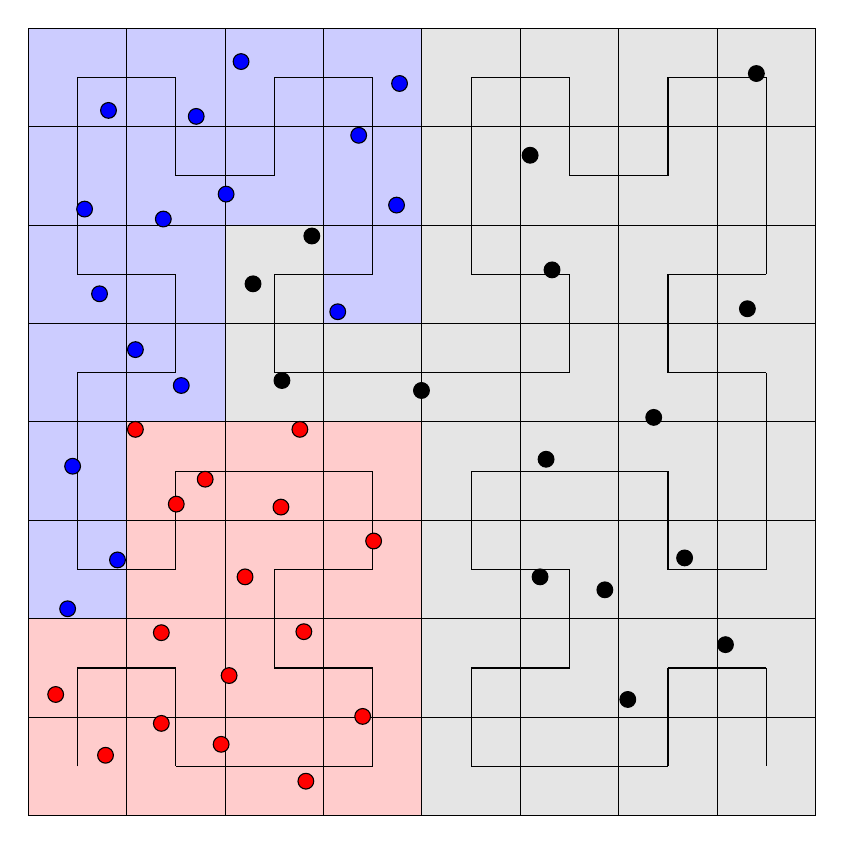
\begin{tikzpicture}
\draw[fill=red!20!white] (0.0, 0.0) rectangle (1.25, 1.25);
\draw[fill=red!20!white] (0.0, 1.25) rectangle (1.25, 2.5);
\draw[fill=red!20!white] (1.25, 1.25) rectangle (2.5, 2.5);
\draw[fill=red!20!white] (1.25, 0.0) rectangle (2.5, 1.25);
\draw[fill=red!20!white] (2.5, 0.0) rectangle (3.75, 1.25);
\draw[fill=red!20!white] (3.75, 0.0) rectangle (5.0, 1.25);
\draw[fill=red!20!white] (3.75, 1.25) rectangle (5.0, 2.5);
\draw[fill=red!20!white] (2.5, 1.25) rectangle (3.75, 2.5);
\draw[fill=red!20!white] (2.5, 2.5) rectangle (3.75, 3.75);
\draw[fill=red!20!white] (3.75, 2.5) rectangle (5.0, 3.75);
\draw[fill=red!20!white] (3.75, 3.75) rectangle (5.0, 5.0);
\draw[fill=red!20!white] (2.5, 3.75) rectangle (3.75, 5.0);
\draw[fill=red!20!white] (1.25, 3.75) rectangle (2.5, 5.0);
\draw[fill=red!20!white] (1.25, 2.5) rectangle (2.5, 3.75);
\draw[fill=blue!20!white] (0.0, 2.5) rectangle (1.25, 3.75);
\draw[fill=blue!20!white] (0.0, 3.75) rectangle (1.25, 5.0);
\draw[fill=blue!20!white] (0.0, 5.0) rectangle (1.25, 6.25);
\draw[fill=blue!20!white] (1.25, 5.0) rectangle (2.5, 6.25);
\draw[fill=blue!20!white] (1.25, 6.25) rectangle (2.5, 7.5);
\draw[fill=blue!20!white] (0.0, 6.25) rectangle (1.25, 7.5);
\draw[fill=blue!20!white] (0.0, 7.5) rectangle (1.25, 8.75);
\draw[fill=blue!20!white] (0.0, 8.75) rectangle (1.25, 10.0);
\draw[fill=blue!20!white] (1.25, 8.75) rectangle (2.5, 10.0);
\draw[fill=blue!20!white] (1.25, 7.5) rectangle (2.5, 8.75);
\draw[fill=blue!20!white] (2.5, 7.5) rectangle (3.75, 8.75);
\draw[fill=blue!20!white] (2.5, 8.75) rectangle (3.75, 10.0);
\draw[fill=blue!20!white] (3.75, 8.75) rectangle (5.0, 10.0);
\draw[fill=blue!20!white] (3.75, 7.5) rectangle (5.0, 8.75);
\draw[fill=blue!20!white] (3.75, 6.25) rectangle (5.0, 7.5);
\draw[fill=gray!20!white] (2.5, 6.25) rectangle (3.75, 7.5);
\draw[fill=gray!20!white] (2.5, 5.0) rectangle (3.75, 6.25);
\draw[fill=gray!20!white] (3.75, 5.0) rectangle (5.0, 6.25);
\draw[fill=gray!20!white] (5.0, 5.0) rectangle (6.25, 6.25);
\draw[fill=gray!20!white] (6.25, 5.0) rectangle (7.5, 6.25);
\draw[fill=gray!20!white] (6.25, 6.25) rectangle (7.5, 7.5);
\draw[fill=gray!20!white] (5.0, 6.25) rectangle (6.25, 7.5);
\draw[fill=gray!20!white] (5.0, 7.5) rectangle (6.25, 8.75);
\draw[fill=gray!20!white] (5.0, 8.75) rectangle (6.25, 10.0);
\draw[fill=gray!20!white] (6.25, 8.75) rectangle (7.5, 10.0);
\draw[fill=gray!20!white] (6.25, 7.5) rectangle (7.5, 8.75);
\draw[fill=gray!20!white] (7.5, 7.5) rectangle (8.75, 8.75);
\draw[fill=gray!20!white] (7.5, 8.75) rectangle (8.75, 10.0);
\draw[fill=gray!20!white] (8.75, 8.75) rectangle (10.0, 10.0);
\draw[fill=gray!20!white] (8.75, 7.5) rectangle (10.0, 8.75);
\draw[fill=gray!20!white] (8.75, 6.25) rectangle (10.0, 7.5);
\draw[fill=gray!20!white] (7.5, 6.25) rectangle (8.75, 7.5);
\draw[fill=gray!20!white] (7.5, 5.0) rectangle (8.75, 6.25);
\draw[fill=gray!20!white] (8.75, 5.0) rectangle (10.0, 6.25);
\draw[fill=gray!20!white] (8.75, 3.75) rectangle (10.0, 5.0);
\draw[fill=gray!20!white] (8.75, 2.5) rectangle (10.0, 3.75);
\draw[fill=gray!20!white] (7.5, 2.5) rectangle (8.75, 3.75);
\draw[fill=gray!20!white] (7.5, 3.75) rectangle (8.75, 5.0);
\draw[fill=gray!20!white] (6.25, 3.75) rectangle (7.5, 5.0);
\draw[fill=gray!20!white] (5.0, 3.75) rectangle (6.25, 5.0);
\draw[fill=gray!20!white] (5.0, 2.5) rectangle (6.25, 3.75);
\draw[fill=gray!20!white] (6.25, 2.5) rectangle (7.5, 3.75);
\draw[fill=gray!20!white] (6.25, 1.25) rectangle (7.5, 2.5);
\draw[fill=gray!20!white] (5.0, 1.25) rectangle (6.25, 2.5);
\draw[fill=gray!20!white] (5.0, 0.0) rectangle (6.25, 1.25);
\draw[fill=gray!20!white] (6.25, 0.0) rectangle (7.5, 1.25);
\draw[fill=gray!20!white] (7.5, 0.0) rectangle (8.75, 1.25);
\draw[fill=gray!20!white] (7.5, 1.25) rectangle (8.75, 2.5);
\draw[fill=gray!20!white] (8.75, 1.25) rectangle (10.0, 2.5);
\draw[fill=gray!20!white] (8.75, 0.0) rectangle (10.0, 1.25);
\draw (0.625, 0.625) -- (0.625, 1.875);
\draw (0.625, 1.875) -- (1.875, 1.875);
\draw (1.875, 1.875) -- (1.875, 0.625);
\draw (1.875, 0.625) -- (3.125, 0.625);
\draw (3.125, 0.625) -- (4.375, 0.625);
\draw (4.375, 0.625) -- (4.375, 1.875);
\draw (4.375, 1.875) -- (3.125, 1.875);
\draw (3.125, 1.875) -- (3.125, 3.125);
\draw (3.125, 3.125) -- (4.375, 3.125);
\draw (4.375, 3.125) -- (4.375, 4.375);
\draw (4.375, 4.375) -- (3.125, 4.375);
\draw (3.125, 4.375) -- (1.875, 4.375);
\draw (1.875, 4.375) -- (1.875, 3.125);
\draw (1.875, 3.125) -- (0.625, 3.125);
\draw (0.625, 3.125) -- (0.625, 4.375);
\draw (0.625, 4.375) -- (0.625, 5.625);
\draw (0.625, 5.625) -- (1.875, 5.625);
\draw (1.875, 5.625) -- (1.875, 6.875);
\draw (1.875, 6.875) -- (0.625, 6.875);
\draw (0.625, 6.875) -- (0.625, 8.125);
\draw (0.625, 8.125) -- (0.625, 9.375);
\draw (0.625, 9.375) -- (1.875, 9.375);
\draw (1.875, 9.375) -- (1.875, 8.125);
\draw (1.875, 8.125) -- (3.125, 8.125);
\draw (3.125, 8.125) -- (3.125, 9.375);
\draw (3.125, 9.375) -- (4.375, 9.375);
\draw (4.375, 9.375) -- (4.375, 8.125);
\draw (4.375, 8.125) -- (4.375, 6.875);
\draw (4.375, 6.875) -- (3.125, 6.875);
\draw (3.125, 6.875) -- (3.125, 5.625);
\draw (3.125, 5.625) -- (4.375, 5.625);
\draw (4.375, 5.625) -- (5.625, 5.625);
\draw (5.625, 5.625) -- (6.875, 5.625);
\draw (6.875, 5.625) -- (6.875, 6.875);
\draw (6.875, 6.875) -- (5.625, 6.875);
\draw (5.625, 6.875) -- (5.625, 8.125);
\draw (5.625, 8.125) -- (5.625, 9.375);
\draw (5.625, 9.375) -- (6.875, 9.375);
\draw (6.875, 9.375) -- (6.875, 8.125);
\draw (6.875, 8.125) -- (8.125, 8.125);
\draw (8.125, 8.125) -- (8.125, 9.375);
\draw (8.125, 9.375) -- (9.375, 9.375);
\draw (9.375, 9.375) -- (9.375, 8.125);
\draw (9.375, 8.125) -- (9.375, 6.875);
\draw (9.375, 6.875) -- (8.125, 6.875);
\draw (8.125, 6.875) -- (8.125, 5.625);
\draw (8.125, 5.625) -- (9.375, 5.625);
\draw (9.375, 5.625) -- (9.375, 4.375);
\draw (9.375, 4.375) -- (9.375, 3.125);
\draw (9.375, 3.125) -- (8.125, 3.125);
\draw (8.125, 3.125) -- (8.125, 4.375);
\draw (8.125, 4.375) -- (6.875, 4.375);
\draw (6.875, 4.375) -- (5.625, 4.375);
\draw (5.625, 4.375) -- (5.625, 3.125);
\draw (5.625, 3.125) -- (6.875, 3.125);
\draw (6.875, 3.125) -- (6.875, 1.875);
\draw (6.875, 1.875) -- (5.625, 1.875);
\draw (5.625, 1.875) -- (5.625, 0.625);
\draw (5.625, 0.625) -- (6.875, 0.625);
\draw (6.875, 0.625) -- (8.125, 0.625);
\draw (8.125, 0.625) -- (8.125, 1.875);
\draw (8.125, 1.875) -- (9.375, 1.875);
\draw (9.375, 1.875) -- (9.375, 0.625);
\draw[fill=red] (0.9816, 0.7664) circle (0.1);
\draw[fill=red] (0.3487, 1.5385) circle (0.1);
\draw[fill=red] (1.6904, 2.3233) circle (0.1);
\draw[fill=red] (1.6904, 1.1714) circle (0.1);
\draw[fill=red] (2.4499, 0.9056) circle (0.1);
\draw[fill=red] (3.5259, 0.4373) circle (0.1);
\draw[fill=red] (4.2474, 1.26) circle (0.1);
\draw[fill=red] (3.5005, 2.336) circle (0.1);
\draw[fill=red] (2.5512, 1.779) circle (0.1);
\draw[fill=red] (2.7537, 3.0322) circle (0.1);
\draw[fill=red] (4.3866, 3.4879) circle (0.1);
\draw[fill=red] (3.2094, 3.9183) circle (0.1);
\draw[fill=red] (3.4499, 4.9056) circle (0.1);
\draw[fill=red] (1.3613, 4.9056) circle (0.1);
\draw[fill=red] (2.2474, 4.2727) circle (0.1);
\draw[fill=red] (1.8803, 3.9562) circle (0.1);
\draw[fill=blue] (1.1335, 3.2474) circle (0.1);
\draw[fill=blue] (0.5005, 2.6271) circle (0.1);
\draw[fill=blue] (0.5638, 4.4373) circle (0.1);
\draw[fill=blue] (1.3613, 5.9183) circle (0.1);
\draw[fill=blue] (1.9436, 5.4626) circle (0.1);
\draw[fill=blue] (0.9056, 6.6271) circle (0.1);
\draw[fill=blue] (0.7157, 7.7031) circle (0.1);
\draw[fill=blue] (1.0195, 8.9562) circle (0.1);
\draw[fill=blue] (2.1335, 8.8803) circle (0.1);
\draw[fill=blue] (1.7157, 7.5765) circle (0.1);
\draw[fill=blue] (2.5132, 7.893) circle (0.1);
\draw[fill=blue] (2.7031, 9.5765) circle (0.1);
\draw[fill=blue] (4.7157, 9.298) circle (0.1);
\draw[fill=blue] (4.6778, 7.7537) circle (0.1);
\draw[fill=blue] (4.1968, 8.6398) circle (0.1);
\draw[fill=blue] (3.9309, 6.3993) circle (0.1);
\draw[fill=black] (2.855, 6.7537) circle (0.1);
\draw[fill=black] (3.6018, 7.3613) circle (0.1);
\draw[fill=black] (3.2221, 5.5259) circle (0.1);
\draw[fill=black] (4.9942, 5.3993) circle (0.1);
\draw[fill=black] (6.6524, 6.9309) circle (0.1);
\draw[fill=black] (6.374, 8.3866) circle (0.1);
\draw[fill=black] (9.2474, 9.4246) circle (0.1);
\draw[fill=black] (9.1335, 6.4373) circle (0.1);
\draw[fill=black] (7.9436, 5.0575) circle (0.1);
\draw[fill=black] (8.336, 3.2727) circle (0.1);
\draw[fill=black] (6.5765, 4.5259) circle (0.1);
\draw[fill=black] (6.5005, 3.0322) circle (0.1);
\draw[fill=black] (7.3233, 2.8676) circle (0.1);
\draw[fill=black] (7.6145, 1.4752) circle (0.1);
\draw[fill=black] (8.855, 2.1714) circle (0.1);

\end{tikzpicture}
\end{document}
% \newpage
\subsection{RQ5: Data Scaling Exploration}

\begin{table}[t]
\caption{A multimodal OOC misinformation detectors with distinct LVLMs. Evaluated on the NewsCLIPpings~\cite{luo2021newsclippings} dataset.}
\centering
\small
% \setlength{\tabcolsep}{0.5pt} % 调整列间距,减小为4pt
% \renewcommand{\arraystretch}{1.1} % 调整行高(默认为1)
    \begin{adjustbox}{valign=c,max width=\columnwidth}
        \begin{tabular}{lc|c|c}
            \toprule
            Settings & Tuning & Parameters & \textbf{All} \\
            \hline
            Random & \xmark & -  & 50.3	\\
            Qwen2-VL-2B & \xmark & 1.5B  & 65.7 \\
            Qwen2-VL-7B & \xmark & 7.6B  &  79.1 \\
            Qwen2-VL-72B & \xmark & 72B  & 79.8 \\
            \hline
            Qwen2-VL-2B & \cmark & 1.5B  & 81.4	\\
            \rowcolor{lightgreen} Qwen2-VL-7B & \cmark & 7.6B  & \textbf{89.9} \\
            \bottomrule
        \end{tabular}
    \end{adjustbox}
\label{tab:tab_4}
\end{table}


\begin{table}[t]
\caption{Comparison on distinct LVLMs between data construction and model tuning. Evaluated on NewsCLIPpings~\cite{luo2021newsclippings}.}
\centering
\small
% \setlength{\tabcolsep}{5.5pt} % 调整列间距,减小为4pt
% \renewcommand{\arraystretch}{1.1} % 调整行高(默认为1)
    \begin{adjustbox}{valign=c,max width=\columnwidth}
        \begin{tabular}{lcl|c}
        \toprule
         Data Construction &  \ding{223} & Model  Tuning & \textbf{All} \\
        \hline
        Qwen2-VL-2B & \ding{223} & Qwen2-VL-2B   & 81.1 \\
        Qwen2-VL-2B & \ding{223} & Qwen2-VL-7B   & 87.6 \\
        \hline
        Qwen2-VL-7B & \ding{223} & Qwen2-VL-2B   & 81.4 \\
        \rowcolor{lightgreen} Qwen2-VL-7B & \ding{223} & Qwen2-VL-7B   & \textbf{89.9} \\
        \bottomrule
        \end{tabular}
    \end{adjustbox}
\label{tab:tab_5}
\end{table}


% \begin{figure}[t]
%   \centering
%    \includegraphics[width=.9\linewidth]{sec/fig6.jpg}
%    \caption{Performance of E2LVM on NewsCLIPpings~\cite{luo2021newsclippings} using different training data proportions.}
%    \label{fig:6}
% \end{figure}

% \newpage
To evaluate the feasibility of rapid deployment of E2LVLM at the stage of early detection, we randomly choose 10$\%$, 25$\%$, 50$\%$, and 75$\%$ samples for experiment analysis. As shown in \Cref{fig:6}, E2LVLM achieves remarkable performance on different proportions of training data. Typically, in a zero-shot scenario, E2LVLM has outperformed the previous method (\eg, DT-Transformer~\cite{papadopoulos2023synthetic}), suggesting the effectiveness of E2LVLM in the task of OOC. With the increasing of samples, the discriminatory powers of E2LVLM have a significant rising tendency. This demonstrates that the proposed E2LVLM can be rapidly deployed and ensure detection accuracy, even at the stage of early detection.

\subsection{RQ6: Robustness Analysis}

% \begin{figure}[t]
%   \centering
%    \includegraphics[width=.9\linewidth]{sec/fig6.jpg}
%    \caption{Performance of E2LVM on NewsCLIPpings~\cite{luo2021newsclippings} using different training data proportions.}
%    \label{fig:6}
% \end{figure}


% \begin{table}[t]
% \caption{Comparison of ``True vs OOC'' accuracy on the dataset VERITE~\cite{papadopoulos2024verite}. Trained on NewsCLIPpings~\cite{luo2021newsclippings} and evaluated on ``All''. The partial results are reported from SNIFFER~\cite{qi2024sniffer}.}
% \centering
% % \Huge
% % \setlength{\tabcolsep}{10pt} % 调整列间距,减小为4pt
% \renewcommand{\arraystretch}{1.1} % 调整行高(默认为1)
%     \begin{adjustbox}{valign=c,max width=\columnwidth}
%         \begin{tabular}{l|c|ll}
%             \toprule
%             Methods & Venue & \textbf{All} & \textbf{True vs OOC} \\
%             \hline
%             RED-DOT~\cite{papadopoulos2023red} & arXiv23 & 84.5 & 73.9 \\
%             SNIFFER~\cite{qi2024sniffer} & CVPR24 & 88.4 ($\uparrow$ 3.9) & 74.0 ($\uparrow$ 0.1)  \\
%             \rowcolor{lightgreen} E2LVLM &  & \textbf{89.9 ($\uparrow$ 5.4)} & \textbf{74.4 ($\uparrow$ 0.5)}  \\
%             \bottomrule
%         \end{tabular}
%     \end{adjustbox}
% \label{tab:tab_6}
% \end{table}

To further verify the robustness of E2LVLM towards real-world scenarios, we implement extended experiments on VERITE~\cite{papadopoulos2024verite}. This dataset serves as a novel real-world OOC misinformation, including 1,000 annotated samples stemming from fact-checking websites. Following~\cite{qi2024sniffer}, we also compare E2LVLM with RED-DOT~\cite{papadopoulos2023red} in \Cref{tab:tab_6}. From the results, we observe that E2LVLM shows the best performance on large-scale NewsCLIPpings~\cite{luo2021newsclippings} and more challenging VERITE~\cite{papadopoulos2024verite}. Typically, E2LVLM achieves a ``True vs OOC'' accuracy of 74.4$\%$, which outperforms RED-DOT by 0.5$\%$ accuracy, and the SOTA SNIFFER by 0.4$\%$ accuracy. The evaluations on these two multimodal OOC misinformation datasets exhibit the detection accuracy and robustness of E2LVLM in practical scenarios.

% \documentclass{standalone}
%\usetikzlibrary{...}
\usepackage{tikz}
\begin{document}
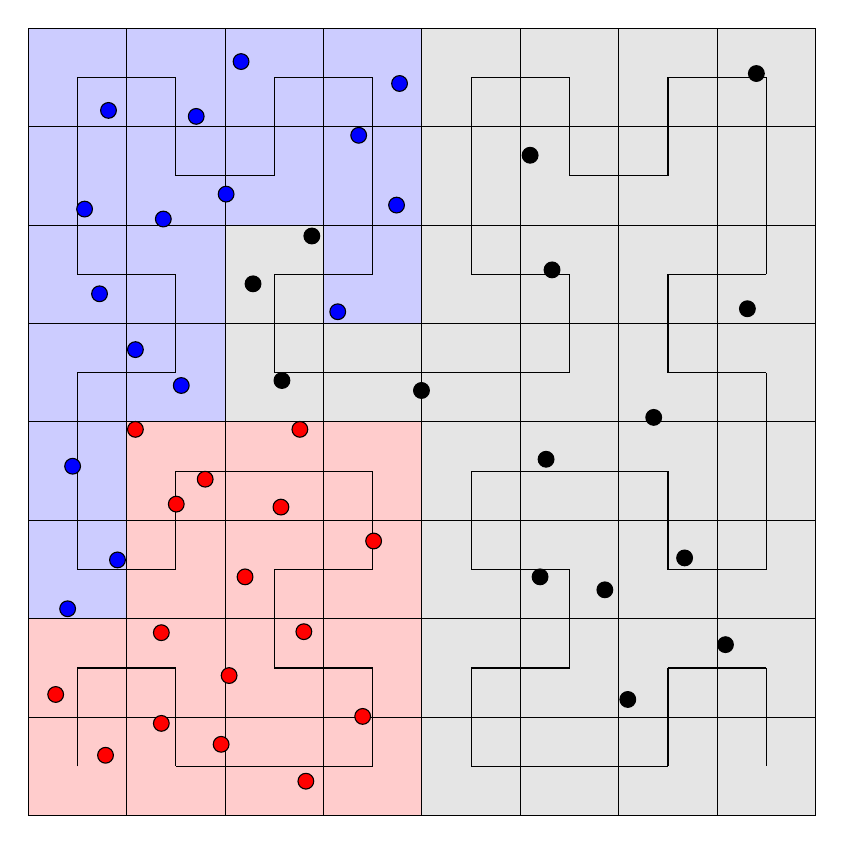
\begin{tikzpicture}
\draw[fill=red!20!white] (0.0, 0.0) rectangle (1.25, 1.25);
\draw[fill=red!20!white] (0.0, 1.25) rectangle (1.25, 2.5);
\draw[fill=red!20!white] (1.25, 1.25) rectangle (2.5, 2.5);
\draw[fill=red!20!white] (1.25, 0.0) rectangle (2.5, 1.25);
\draw[fill=red!20!white] (2.5, 0.0) rectangle (3.75, 1.25);
\draw[fill=red!20!white] (3.75, 0.0) rectangle (5.0, 1.25);
\draw[fill=red!20!white] (3.75, 1.25) rectangle (5.0, 2.5);
\draw[fill=red!20!white] (2.5, 1.25) rectangle (3.75, 2.5);
\draw[fill=red!20!white] (2.5, 2.5) rectangle (3.75, 3.75);
\draw[fill=red!20!white] (3.75, 2.5) rectangle (5.0, 3.75);
\draw[fill=red!20!white] (3.75, 3.75) rectangle (5.0, 5.0);
\draw[fill=red!20!white] (2.5, 3.75) rectangle (3.75, 5.0);
\draw[fill=red!20!white] (1.25, 3.75) rectangle (2.5, 5.0);
\draw[fill=red!20!white] (1.25, 2.5) rectangle (2.5, 3.75);
\draw[fill=blue!20!white] (0.0, 2.5) rectangle (1.25, 3.75);
\draw[fill=blue!20!white] (0.0, 3.75) rectangle (1.25, 5.0);
\draw[fill=blue!20!white] (0.0, 5.0) rectangle (1.25, 6.25);
\draw[fill=blue!20!white] (1.25, 5.0) rectangle (2.5, 6.25);
\draw[fill=blue!20!white] (1.25, 6.25) rectangle (2.5, 7.5);
\draw[fill=blue!20!white] (0.0, 6.25) rectangle (1.25, 7.5);
\draw[fill=blue!20!white] (0.0, 7.5) rectangle (1.25, 8.75);
\draw[fill=blue!20!white] (0.0, 8.75) rectangle (1.25, 10.0);
\draw[fill=blue!20!white] (1.25, 8.75) rectangle (2.5, 10.0);
\draw[fill=blue!20!white] (1.25, 7.5) rectangle (2.5, 8.75);
\draw[fill=blue!20!white] (2.5, 7.5) rectangle (3.75, 8.75);
\draw[fill=blue!20!white] (2.5, 8.75) rectangle (3.75, 10.0);
\draw[fill=blue!20!white] (3.75, 8.75) rectangle (5.0, 10.0);
\draw[fill=blue!20!white] (3.75, 7.5) rectangle (5.0, 8.75);
\draw[fill=blue!20!white] (3.75, 6.25) rectangle (5.0, 7.5);
\draw[fill=gray!20!white] (2.5, 6.25) rectangle (3.75, 7.5);
\draw[fill=gray!20!white] (2.5, 5.0) rectangle (3.75, 6.25);
\draw[fill=gray!20!white] (3.75, 5.0) rectangle (5.0, 6.25);
\draw[fill=gray!20!white] (5.0, 5.0) rectangle (6.25, 6.25);
\draw[fill=gray!20!white] (6.25, 5.0) rectangle (7.5, 6.25);
\draw[fill=gray!20!white] (6.25, 6.25) rectangle (7.5, 7.5);
\draw[fill=gray!20!white] (5.0, 6.25) rectangle (6.25, 7.5);
\draw[fill=gray!20!white] (5.0, 7.5) rectangle (6.25, 8.75);
\draw[fill=gray!20!white] (5.0, 8.75) rectangle (6.25, 10.0);
\draw[fill=gray!20!white] (6.25, 8.75) rectangle (7.5, 10.0);
\draw[fill=gray!20!white] (6.25, 7.5) rectangle (7.5, 8.75);
\draw[fill=gray!20!white] (7.5, 7.5) rectangle (8.75, 8.75);
\draw[fill=gray!20!white] (7.5, 8.75) rectangle (8.75, 10.0);
\draw[fill=gray!20!white] (8.75, 8.75) rectangle (10.0, 10.0);
\draw[fill=gray!20!white] (8.75, 7.5) rectangle (10.0, 8.75);
\draw[fill=gray!20!white] (8.75, 6.25) rectangle (10.0, 7.5);
\draw[fill=gray!20!white] (7.5, 6.25) rectangle (8.75, 7.5);
\draw[fill=gray!20!white] (7.5, 5.0) rectangle (8.75, 6.25);
\draw[fill=gray!20!white] (8.75, 5.0) rectangle (10.0, 6.25);
\draw[fill=gray!20!white] (8.75, 3.75) rectangle (10.0, 5.0);
\draw[fill=gray!20!white] (8.75, 2.5) rectangle (10.0, 3.75);
\draw[fill=gray!20!white] (7.5, 2.5) rectangle (8.75, 3.75);
\draw[fill=gray!20!white] (7.5, 3.75) rectangle (8.75, 5.0);
\draw[fill=gray!20!white] (6.25, 3.75) rectangle (7.5, 5.0);
\draw[fill=gray!20!white] (5.0, 3.75) rectangle (6.25, 5.0);
\draw[fill=gray!20!white] (5.0, 2.5) rectangle (6.25, 3.75);
\draw[fill=gray!20!white] (6.25, 2.5) rectangle (7.5, 3.75);
\draw[fill=gray!20!white] (6.25, 1.25) rectangle (7.5, 2.5);
\draw[fill=gray!20!white] (5.0, 1.25) rectangle (6.25, 2.5);
\draw[fill=gray!20!white] (5.0, 0.0) rectangle (6.25, 1.25);
\draw[fill=gray!20!white] (6.25, 0.0) rectangle (7.5, 1.25);
\draw[fill=gray!20!white] (7.5, 0.0) rectangle (8.75, 1.25);
\draw[fill=gray!20!white] (7.5, 1.25) rectangle (8.75, 2.5);
\draw[fill=gray!20!white] (8.75, 1.25) rectangle (10.0, 2.5);
\draw[fill=gray!20!white] (8.75, 0.0) rectangle (10.0, 1.25);
\draw (0.625, 0.625) -- (0.625, 1.875);
\draw (0.625, 1.875) -- (1.875, 1.875);
\draw (1.875, 1.875) -- (1.875, 0.625);
\draw (1.875, 0.625) -- (3.125, 0.625);
\draw (3.125, 0.625) -- (4.375, 0.625);
\draw (4.375, 0.625) -- (4.375, 1.875);
\draw (4.375, 1.875) -- (3.125, 1.875);
\draw (3.125, 1.875) -- (3.125, 3.125);
\draw (3.125, 3.125) -- (4.375, 3.125);
\draw (4.375, 3.125) -- (4.375, 4.375);
\draw (4.375, 4.375) -- (3.125, 4.375);
\draw (3.125, 4.375) -- (1.875, 4.375);
\draw (1.875, 4.375) -- (1.875, 3.125);
\draw (1.875, 3.125) -- (0.625, 3.125);
\draw (0.625, 3.125) -- (0.625, 4.375);
\draw (0.625, 4.375) -- (0.625, 5.625);
\draw (0.625, 5.625) -- (1.875, 5.625);
\draw (1.875, 5.625) -- (1.875, 6.875);
\draw (1.875, 6.875) -- (0.625, 6.875);
\draw (0.625, 6.875) -- (0.625, 8.125);
\draw (0.625, 8.125) -- (0.625, 9.375);
\draw (0.625, 9.375) -- (1.875, 9.375);
\draw (1.875, 9.375) -- (1.875, 8.125);
\draw (1.875, 8.125) -- (3.125, 8.125);
\draw (3.125, 8.125) -- (3.125, 9.375);
\draw (3.125, 9.375) -- (4.375, 9.375);
\draw (4.375, 9.375) -- (4.375, 8.125);
\draw (4.375, 8.125) -- (4.375, 6.875);
\draw (4.375, 6.875) -- (3.125, 6.875);
\draw (3.125, 6.875) -- (3.125, 5.625);
\draw (3.125, 5.625) -- (4.375, 5.625);
\draw (4.375, 5.625) -- (5.625, 5.625);
\draw (5.625, 5.625) -- (6.875, 5.625);
\draw (6.875, 5.625) -- (6.875, 6.875);
\draw (6.875, 6.875) -- (5.625, 6.875);
\draw (5.625, 6.875) -- (5.625, 8.125);
\draw (5.625, 8.125) -- (5.625, 9.375);
\draw (5.625, 9.375) -- (6.875, 9.375);
\draw (6.875, 9.375) -- (6.875, 8.125);
\draw (6.875, 8.125) -- (8.125, 8.125);
\draw (8.125, 8.125) -- (8.125, 9.375);
\draw (8.125, 9.375) -- (9.375, 9.375);
\draw (9.375, 9.375) -- (9.375, 8.125);
\draw (9.375, 8.125) -- (9.375, 6.875);
\draw (9.375, 6.875) -- (8.125, 6.875);
\draw (8.125, 6.875) -- (8.125, 5.625);
\draw (8.125, 5.625) -- (9.375, 5.625);
\draw (9.375, 5.625) -- (9.375, 4.375);
\draw (9.375, 4.375) -- (9.375, 3.125);
\draw (9.375, 3.125) -- (8.125, 3.125);
\draw (8.125, 3.125) -- (8.125, 4.375);
\draw (8.125, 4.375) -- (6.875, 4.375);
\draw (6.875, 4.375) -- (5.625, 4.375);
\draw (5.625, 4.375) -- (5.625, 3.125);
\draw (5.625, 3.125) -- (6.875, 3.125);
\draw (6.875, 3.125) -- (6.875, 1.875);
\draw (6.875, 1.875) -- (5.625, 1.875);
\draw (5.625, 1.875) -- (5.625, 0.625);
\draw (5.625, 0.625) -- (6.875, 0.625);
\draw (6.875, 0.625) -- (8.125, 0.625);
\draw (8.125, 0.625) -- (8.125, 1.875);
\draw (8.125, 1.875) -- (9.375, 1.875);
\draw (9.375, 1.875) -- (9.375, 0.625);
\draw[fill=red] (0.9816, 0.7664) circle (0.1);
\draw[fill=red] (0.3487, 1.5385) circle (0.1);
\draw[fill=red] (1.6904, 2.3233) circle (0.1);
\draw[fill=red] (1.6904, 1.1714) circle (0.1);
\draw[fill=red] (2.4499, 0.9056) circle (0.1);
\draw[fill=red] (3.5259, 0.4373) circle (0.1);
\draw[fill=red] (4.2474, 1.26) circle (0.1);
\draw[fill=red] (3.5005, 2.336) circle (0.1);
\draw[fill=red] (2.5512, 1.779) circle (0.1);
\draw[fill=red] (2.7537, 3.0322) circle (0.1);
\draw[fill=red] (4.3866, 3.4879) circle (0.1);
\draw[fill=red] (3.2094, 3.9183) circle (0.1);
\draw[fill=red] (3.4499, 4.9056) circle (0.1);
\draw[fill=red] (1.3613, 4.9056) circle (0.1);
\draw[fill=red] (2.2474, 4.2727) circle (0.1);
\draw[fill=red] (1.8803, 3.9562) circle (0.1);
\draw[fill=blue] (1.1335, 3.2474) circle (0.1);
\draw[fill=blue] (0.5005, 2.6271) circle (0.1);
\draw[fill=blue] (0.5638, 4.4373) circle (0.1);
\draw[fill=blue] (1.3613, 5.9183) circle (0.1);
\draw[fill=blue] (1.9436, 5.4626) circle (0.1);
\draw[fill=blue] (0.9056, 6.6271) circle (0.1);
\draw[fill=blue] (0.7157, 7.7031) circle (0.1);
\draw[fill=blue] (1.0195, 8.9562) circle (0.1);
\draw[fill=blue] (2.1335, 8.8803) circle (0.1);
\draw[fill=blue] (1.7157, 7.5765) circle (0.1);
\draw[fill=blue] (2.5132, 7.893) circle (0.1);
\draw[fill=blue] (2.7031, 9.5765) circle (0.1);
\draw[fill=blue] (4.7157, 9.298) circle (0.1);
\draw[fill=blue] (4.6778, 7.7537) circle (0.1);
\draw[fill=blue] (4.1968, 8.6398) circle (0.1);
\draw[fill=blue] (3.9309, 6.3993) circle (0.1);
\draw[fill=black] (2.855, 6.7537) circle (0.1);
\draw[fill=black] (3.6018, 7.3613) circle (0.1);
\draw[fill=black] (3.2221, 5.5259) circle (0.1);
\draw[fill=black] (4.9942, 5.3993) circle (0.1);
\draw[fill=black] (6.6524, 6.9309) circle (0.1);
\draw[fill=black] (6.374, 8.3866) circle (0.1);
\draw[fill=black] (9.2474, 9.4246) circle (0.1);
\draw[fill=black] (9.1335, 6.4373) circle (0.1);
\draw[fill=black] (7.9436, 5.0575) circle (0.1);
\draw[fill=black] (8.336, 3.2727) circle (0.1);
\draw[fill=black] (6.5765, 4.5259) circle (0.1);
\draw[fill=black] (6.5005, 3.0322) circle (0.1);
\draw[fill=black] (7.3233, 2.8676) circle (0.1);
\draw[fill=black] (7.6145, 1.4752) circle (0.1);
\draw[fill=black] (8.855, 2.1714) circle (0.1);

\end{tikzpicture}
\end{document}